\documentclass[12pt,a4paper,notitlepage,twocolumn,oneside]{article}
\usepackage[utf8x]{inputenc}
\usepackage{ucs}
\usepackage{amsmath}
\usepackage{amsfonts}
\usepackage{amssymb}
\usepackage{graphicx}
\usepackage{hyperref}

\usepackage[dvips]{color} 
\definecolor{darkblue}{rgb}{0,0,.3}
\definecolor{darkgreen}{rgb}{0,.3,0}
\definecolor{darkred}{rgb}{.3,0,0}
\hypersetup{%
	colorlinks=true,
	linkcolor=darkblue,
	menucolor=darkblue,
	pagecolor=darkblue,
	urlcolor=darkblue,
	citecolor=darkgreen,
	filecolor=darkred
}

\hypersetup{
	pdftitle={Atomic Tagging},
	pdfauthor={Stephan Mann},
	pdfsubject={Atomic Tagging},
	pdfkeywords={information management, tags, delicious}
}

\newcommand{\at}{{\emph{Atomic Tagging}}}

\author{Stephan Mann}
\title{Atomic Tagging}
\date{2010-02-04}

\begin{document}
\maketitle


%%%%%%%%%%%%%%%%%%%%%%%%%%%%%% SECTION %%%%%%%%%%%%%%%%%%%%%%%%%%%%%%

\section*{Abstract}
The smallest container a common desktop system can store data in is a file. Files in turn are managed in a directory structure. This structure is very versatile and easy to understand for users, but it has many constraints for the data management and offers very little support for information management. 

Many applications, on the desktop and the web, introduced an abstraction layer to be able to manage smaller parts of data or to enable better management of meta data. Most of the time, these applications manage a single very specific type of data, like bookmarks, images or audio files.

This paper describes an alternative way of managing data to enable information management. By breaking up data into much smaller parts, giving up the distinction between data and meta data and the use of tagging instead of a directory structure, a comparably homogeneous but much more flexible environment can be created. It can be used as a universal system to manage data and information of any kind, not just a single type. 

The paper then describes what additional value could be created by a specific implementation of this system.


%%%%%%%%%%%%%%%%%%%%%%%%%%%%%% SECTION %%%%%%%%%%%%%%%%%%%%%%%%%%%%%%

\section{Introduction}
\subsection{Operating and file systems}\label{op_file_systems}
Common operating systems offer support only for data management. Most of the time, the possibilities of their underlying file system show through nearly unfiltered. File systems provide a hierarchical structure for files and directories and some additional attributes. The simplicity and versatility of this hierarchical structure offers very good data management, even for unforeseen applications, and the file/folder metaphor is easy to understand for users.

But computer systems are supposed to manage information, not mere data. Little support is offered by the operating system or the file system to accomplish that task. To manage information, meta data is required and needs to be managed. The lacking support from operating systems and file systems has spawned an uncountable number of information management applications, most of them implementing their own way of meta data (and thus information) management by introducing an abstraction layer in one form or another. This in turn led to many incompatible meta data formats and storing technologies. Some use a single file, others a database of some kind. Most of the time, these applications are not compatible to one another and the information can be retrieved only if the right application is used.

What is required, is an simple and versatile structure for managing information. It must be flexible enough to be used even for unforeseen applications and the metaphor must be easily understood by the user or offer the possibility, to be completely hidden from the users eye.

\subsection{Data vs. Information}
To turn data into information, a context is required. The number "080012345555" on its own holds no information. Only with the additional data of "phone number" and a link between the data sets, it is useful to computer systems and users. This additional data is called meta data.

The same effect can be accomplished by using a syntax of some kind. But while it is sufficient for some data like an URL (e.g. "http://www.example.com") to be meaningful, it is insufficient for other data like the previous example. Even when put into the international syntax, the string "+49 800 12 34 5555" still could mean a phone or a fax number. It is therefor better to store the context explicitly and not to encode it (only) into the syntax. 

Some file formats offer the possibility to link additional meta data to one data set not just to be able to use the latter at all, but to increase the informational value. A common example are the ID3v2 frames\footnote{ID3v2 specification - \url{http://www.id3.org/id3v2.4.0-frames}} for MP3 files which provide the means to add artist or genre data to an MP3 file. To read this information, an application must implement this specification.

As described in section \ref{op_file_systems}, file systems themselves offer very little support for meta data. The context can be encoded in the location of a file, showing that it belongs to a certain application. There is also the common convention of using the file name to encode meta data in form of the file extension, the part of the file name after the last dot. Microsoft Windows uses this mainly to link a file to an application. Neither of these conventions can be enforced and the file extension is often replaced by a generic placeholder like "txt" or "dat".

Many applications differentiate between data and meta data and store the first in the file system while they store the latter in an application specific format in a single file or a database. As described in section \ref{atomic_tagging}, \at\ will use a different approach.

\subsection{Shortcomings}\label{shortcomings}
Due to the lacking support for information management by common operating and file systems, many applications implemented their own way of information management. Some of the shortcomings that exist today originated from the first, some from the latter. 

\begin{itemize}
\item The file system shows only the directory structure and the file name. A specific application is required to interpret (binary) data and possibly enclosed meta data. If that application is not available, the user is left with an unusable data blob and can not even access the meta data.
\item Every file type that supports the storage of meta data does so in its own way, like MP3's ID3v2 or EXIF\footnote{EXIF - \url{http://www.exif.org/}} for image files. Adobe's XMP\footnote{Extensible Metadata Platform - \url{http://www.adobe.com/devnet/xmp/pdfs/xmp_specification.pdf}} tries to specify a common format for the storage of meta data but has not been adopted beyond the PDF file format.
\item Since meta data is stored inside the files, searching meta data becomes very expensive, because all the files need to be read. It is also hard to manage data and meta data apart from each other. Although there are specialized file systems like SAM-QFS\footnote{SAM-QFS - \url{http://hub.opensolaris.org/bin/view/Project+samqfs/WebHome}} that support this, this is not a widely available feature.
\item Some specifications for meta data storage are very limited. For example, the ID3v2 frames for MP3 files support only one genre for an audio file with no possibility to add more resulting in user defined genre strings that combine multiple genres thereby breaking the possibility to do effective searches.
\item There are many applications that can manage a very specific type of data (like audio files or images), but almost none that can manage multiple types of data.
\item There are various types of data for which no application exists to manage it. The attempt to manage them in the file system results in duplicated files or a confusing collection of symbolic links which is tedious to keep up to date.
\item Every application that is able to manage a certain type of data brings its own look and feel. Some applications have created look and feels, that where adopted, but often a user has to learn how to use a certain application anew.
\item Even applications, that do the same (like manage audio files), have their own internal database. If another application is to be used to manage the same information, a new database is required.
\item Advanced functionality is missing. For example, there is no inherent version support resulting in users copying files and putting dates into the file name. Some applications try to compensate, like office bundles or the F-Spot photo manager, all creating their own way of version control.
\end{itemize}

\subsection{Goals}\label{goals}
Following from the shortcomings and a general discontent with the possibilities offered by common desktop systems, this paper tries to depict a new way of information management. The goal is to

\begin{itemize}
\item Find a new metaphor that is as easy to understand as the file/folder metaphor but focuses on information management rather than data management.
\item Erase the shortcomings described in section \ref{shortcomings} by recognizing meta data as an important part of the data which can be accessed independently from the data itself.
\item Design the system so that all data exists in a homogeneous format that can be managed the same way.
\item Build a flexible system where the user can decide how he wants to manage his information.
\end{itemize}


%%%%%%%%%%%%%%%%%%%%%%%%%%%%%% SECTION %%%%%%%%%%%%%%%%%%%%%%%%%%%%%%

\section{Atomic Tagging}\label{atomic_tagging}
During the rise of the so called Web 2.0, a new method for information management has come forward: tagging. Tags are user defined strings, that can be linked to data thus improving the informational value. A user can attach any number of tags to a data set and can then query the system for data with a certain tag. That way, users can create groups of data, while any data can belong to any number of groups without the need to be duplicated.

Delicious\footnote{Delicious - \url{http://del.icio.us}}, a web application for bookmark management, used tagging as one of the first and the obvious superiority in comparison to a hierarchical structure led to the use of tagging all over the web and even in some desktop applications. But tagging works only that well, if there is one specific type of information to manage. Taking this concept to the file system would mean various technical problems (as described in section \ref{file_system}) and would not solve all of the problems described in section \ref{shortcomings}. Tagging files would help a user to better organize the information, but would still mean that many data exists multiple times, because a file contains many data, that can not be individually addressed from the outside.

\at\ therefore takes another step, additionally to using tags. It breaks up data into atoms, the smallest possible part, thus allowing to tag a very specific part of it. It then uses a structure called molecules to link atoms to one another thus creating the context which exists as an address data set or a file. The distinction between data and meta data is erased although it still exists logical, it no longer makes a difference for the underlying system. It's all just atoms. Both atoms and molecules can be tagged to give meaning to the connections and to give the user the possibility, to create groups of data just as in a Web 2.0 application. The main difference is, that this works for every kind of data, not just one specific kind at the time.

\subsection{Atoms}\label{atoms}
Data and meta data is stored in atoms. The size of atoms is subject to the users definition but the system becomes more flexible and the data more reusable with smaller atoms. To reach the maximum flexibility, an atom should contain the smallest possible data, but it might become apparent through use that it is not always wise to fragment the data to the maximum possible. 

The data describing the address of Homer Simpson could be represented by four atoms, shown in table \ref{homer_simpson} with their atom ID, their data and one of their tags.

\begin{table}[htp]
\centering
\begin{tabular}{|c|l|l|}
\hline
\textbf{AID} & \textbf{Data} & \textbf{Tags} \\
\hline
001 & Homer Simpson & name \\
002 & 742 Evergreen Terrace & address \\
003 & Springfield & city \\
004 & USA & country \\
\hline
\end{tabular}
\caption{An address in four atoms}
\label{homer_simpson}
\end{table}

Binary data can be stored in an atom as well, although this will be subject to implementational details in section \ref{compatibility}. Table \ref{image_file} shows an image file with additional meta data describing what the image shows and with what kind of camera it was taken.

\begin{table}[htp]
\centering
\begin{tabular}{|c|l|l|}
\hline
\textbf{AID} & \textbf{Data} & \textbf{Tags} \\
\hline
011 & [binary data] & image \\
012 & Bart Simpson & name \\
013 & Milhouse & name \\
014 & Bart's birthday & event \\
015 & Canon 450D & camera-model \\
016 & 0.25s & camera-time \\
017 & f5.6 & camera-focal \\
\hline
\end{tabular}
\caption{An image file and some meta data in atoms}
\label{image_file}
\end{table}

Fragmenting data this way results in a heterogeneous cloud of data in a homogeneous format. Immediately, the data becomes more reusable. Only one atom containing the camera model is necessary, no matter how many pictures where taken with this camera and every picture Bart Simpson appears on can link to his name atom. And if Bart's address is to be stored, all the data is already there from Homer's address from the previous example. It just needs to get linked.

\subsection{Molecules}\label{molecules}
The problem that arises from the fragmentation of data into atoms is that a data atom, though described by its linked meta data, is missing its context thus loosing information. This loss can be compensated by implementing a logical structure that binds a number of data atoms together.

Molecules are what brings order to the cloud of atoms. They provide the links between atoms thus putting them into context to one another.

\begin{table}[htp]
\centering
\begin{tabular}{|c||c|}
\hline
Molecule 1 & Molecule 2 \\
\hline
\textbf{AtomID} & \textbf{AtomID} \\
\hline
001 & 012 \\
002 & 002 \\
003 & 003 \\
004 & 004 \\
\hline
\end{tabular}

\caption{The addresses of Homer and Bart as molecules}
\label{addresses_simpsons}
\end{table}

As shown by table \ref{addresses_simpsons}, molecules themselves do not contain data. They simply contain links to atoms. They are, however, tagable, providing a second layer of tagging on a higher level.

Any atom can be linked to another thus obtaining meta data. While this first and foremost creates a state where existing data structures like a file or an address card can be reproduced into with \at{,} it also allows for reuse of atoms for multiple molecules. To take the example of an image file from table \ref{image_file}, there is now only one meta data molecule necessary to hold a certain camera model, which then can be linked to all images.

Through the reuse of atoms search becomes very cheap. Searching for an image that was taken with a certain camera model is only to find all molecules that link to that atom. 

Through the simple nature of molecules, defining them is very easy. Table \ref{molecule_definition} shows how a molecule definition could look like.

\begin{table}[htp]
\centering
\begin{tabular}{|l|c|c|}
\hline
\multicolumn{3}{|c|}{\textbf{Molecule "image"}} \\
\hline
\textbf{Tag} & \textbf{Quantity} & \textbf{required} \\
\hline
image & 1 & yes \\
photographer & 1 & no \\
name & * & no \\
camera-model & 1 & no \\
\ldots & \ldots & \ldots \\
\hline
\end{tabular}
\caption{Molecule definition}
\label{molecule_definition}
\end{table}

A molecule is complete, if all requirements have been satisfied by a link to a atom tagged with the specified tag. A molecule could even link to a atom multiple times as described in section \ref{tags_types}.

\subsection{Tags and types}\label{tags_types}
Tags are just user-specified strings attached to data, as described in section \ref{atomic_tagging}. The user could create a tag "favorite pictures" and attach it to any number of image molecules or directly to the the binary data atom.

Considering molecules and their definition, tags serve another purpose as well. They act as a type, allowing them to be linked to a molecule, if they match the molecules definition. Since tags can be added to an atom without quantity restriction, it is possible to have the atom "Bart Simpson" both tagged with "name" and "photographer" and link to it both times in an image molecule.

\subsection{Summary}
Using the proposed system of \at\ to store data creates a homogeneous state in which every atom can be managed the same way. The exception of course are binary data atoms, that need to be handled specifically if they are to be displayed. Through the higher fragmentation of the the data, a much denser net of links can be created increasing reuse of data and the informational value of the system as a whole. 

The possibility of linking everything with everything and the simplicity of the molecules definition allows users to be much more creative on how they want to manage their data.


%%%%%%%%%%%%%%%%%%%%%%%%%%%%%% SECTION %%%%%%%%%%%%%%%%%%%%%%%%%%%%%%

\section{Implementation}\label{implementation}
Even though the described content is environment agnostic and could be implemented as a web application, this paper will focus on its implementation as a desktop application. The concept is designed to manage all data a user has on his PC and until the Internet transfer speeds and data privacy make real progress, this data won't find its way into the Internet as a whole.

\subsection{File system}\label{file_system}
There are a number of projects which try to add tagging support to an operating system, either by wrapping file system operations\footnote{tag(1): del.icio.us-style file tagging - \url{http://blueslugs.com/wordpress/2005/07/12/tag1-delicious-style-file-tagging/}} or by extending already existing functionality of an application that is used by default on this operating system\footnote{XTagFS: A tag-based filesystem for Mac OS X - \url{http://code.google.com/p/xtagfs/}}.

But this approach contains a number of problems. First, it has to handle the combinatoric as described by the \emph{tag(1)} project, which will, eventually, meet the limits of every file system. This constraint would become even more apparent, if \at\ was implemented on the file system, because the atoms would have to be stored into single files. Second, it does not solve the other shortcomings described in \ref{shortcomings}. 

Data can be searched much faster if it is atomic and if it is stored in a database. Writing the molecules to a file system would defeat part of the purpose.

\subsection{Database model}
Therefor, the obvious approach is to implement \at\ on top of a database. Figure \ref{dbmodel} shows a very simple relational database model, that implements the described structure in only six tables. A database has no problems with the combinatoric, since every link is just a new line in one of the tables. While selecting all atoms an molecules with a specific tag is as easy as in the \emph{tag(1)} approach, additionally, full text search becomes very cheap and there is no background process, that needs to update links or tags.

\begin{figure}[ht]
\centering
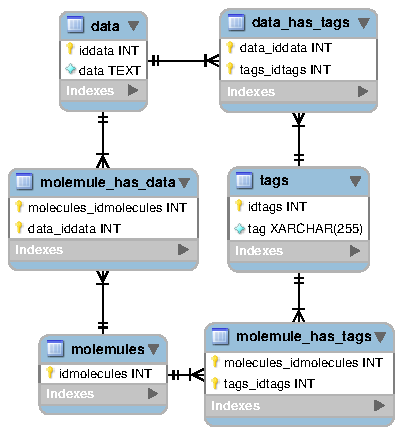
\includegraphics{dbmodel.pdf}
\caption{Database model}
\label{dbmodel}
\end{figure}

\subsection{Compatibility}\label{compatibility}
The problem with any fundamentally new approach for data or information management is, that it won't be adopted, until there are applications for a wide variety of use cases. That is one of the reasons, why there are so many projects trying to add tagging to the file system without breaking the file systems normal behavior, thus keeping compatibility to all other applications.

\at\ is not compatible to a normal file based organization. But compatibility to most applications can be established, by a simple implementation detail, that is also beneficial from the databases point of view. Storing binary data in the database would constitute a problem for the database, because the data field inside the atoms table (see figure \ref{dbmodel}) would have to be "binary" instead of "text". By this, the database would loose the ability to do effective full text searches on the data fields and would have to store text in a binary field. 

The better way to implement this is to store just a reference to a binary file on the underlying file system. Thus, the file still exists and can be handled with the appropriate application (e.g. an image manipulation application).

This approach does not solve the problem for all applications, which handle only plain text data, like an email or address management application. It does however make it possible to use all the specialized application that are not easily reimplemented and leaves just a number of generic applications to be reimplemented on top of \at{.}

\subsection{Molecule browser}\label{molecule_browser}
A browser application similar to a file browser present in most operating systems is easily implemented. Instead of directories and files, now molecules and atoms are shown. A tree-like structure can be created, showing all tags on the first level, removing all atoms and molecules from the subsequent level, that are not tagged with the selected tag. This concept is already demonstrated by the Delicious Firefox Add-on\footnote{Delicious Firefox Add-on - \url{http://delicious.com/help/quicktour/firefox}}.

\subsection{Query language}\label{query_language}
A query language can be implemented equally easy. Just like the molecule browser, it could represent tags as directories, yielding the same result of molecules and atoms despite the order of the tags. So the following two queries would create the same result of favorite music:

\begin{itemize}
\item \texttt{/music/favorite}
\item \texttt{/favorite/music}
\end{itemize}

\subsection{Additional advantages}
Atoms and molecules exist in a homogeneous structure as described in section \ref{atomic_tagging}. Based on this fact a number of new approaches could be implemented to manage data and information.

\subsubsection{Viewers and customized applications}
Because of the homogeneous structure of \at{,} most of the data can be viewed in a generic way in form of a table or another appropriate structure. But for some molecules, especially those containing a binary data atom, special viewers will be required. These viewers can be implemented as stand alone applications, creating one viewer for one specific type of molecule.

Combined with an instance of a molecule browser (see section \ref{molecule_browser}) and the query language (see section \ref{query_language}), additional value could be created: Users could create their own applications. If a set of viewers is available to the system, an application is just a set of queries specifying what data should be visible inside it. An instance of the molecule browser could then show all data matching the query, viewing it with the appropriate viewer modules upon selection. This way, conflicts like whether RSS feeds should be displayed inside a web browser, an email application or in a stand alone application could finally come to an end. It would be the users choice to include the appropriate query into the application specification or not.

\subsubsection{Lists}
Additional data structures could be created. Like molecules, a list data type would be possible, allowing to create lists of atoms or molecules. The definition would vary only slightly from the molecules definition, in that most of the time it will be a list of only one type which has an order.

Using this feature, play lists from the music collection could be created in the same way as a picture set. Different data types could be mixed, if the type tag is chosen wide enough, allowing to mix photographs and videos in one presentation. There is no application switch involved, as long as there are viewers for every molecule in the list.

\subsubsection{Replication and data splitting}
Implementing a data management system on top of a database adds all the features of a database management system (DBMS) to the options of data management. One example is replication. With a DBMS it is possible to set up real time replication, thus ensuring access from another host or backup in event of hardware failure.

With the describe implementation it is also easy to move binary data to another host and to store just the meta data on the main machine. A tag or special atom than could describe what host the binary data resides on or what CD must be inserted to access the binary data.

\subsubsection{Versions}
Version management can be done in the same way for all data. A molecule super-seeding another can link to the old molecule and vice versa. In that way, all molecules that are super-seeded can be removed from view while new molecules retain the possibility to retrieve old versions. Version management can be done effectively because only the changed atoms need to be created and linked to the new molecule. The old ones just are linked again.


%%%%%%%%%%%%%%%%%%%%%%%%%%%%%% SECTION %%%%%%%%%%%%%%%%%%%%%%%%%%%%%%

\section{Conclusion}
The goals described in section \ref{goals} could be achieved with an implementation of \at{.} Also, the shortcomings described in section \ref{shortcomings} could be fixed. 

\begin{itemize}
\item All plain text data can be interpreted in the same generic way. 
\item There is only one format for meta data and it is easily accessible even if the binary file can not be interpreted on the system.
\item Full text search and meta data search becomes very cheap.
\item Meta data can be extended by the user and is no longer restricted to any specification. 
\item Database features (as implemented by some applications) are now part of the underlying system an apply to all applications.
\item Building user customized applications becomes very easy.
\item All applications handle the same way. If a new feature is implemented, it applies to all of them.
\item Advanced functionality like version management can be implemented.
\end{itemize}

\at\ provides a system that is versatile enough to allow for the implementation of all kinds of information management. The big difference is, that it can be done inside a homogeneous system and needs no workaround inside some container.

\end{document}
